\documentclass[12pt]{report} % You can use 'article' or 'book' class as well

% Set up the page
% \usepackage{multicol}
\usepackage{tabularx}
\usepackage{listings}
\usepackage{titlesec}
\usepackage{tocloft}
\usepackage{hyperref} % For clickable links
\usepackage[a4paper, total={6in, 8in}]{geometry} % Adjust the margins
\usepackage{amsmath, amssymb} % For mathematical symbols
\usepackage{graphicx} % For including images
\usepackage{lipsum} % To generate filler text for sample sections
\usepackage{fancyhdr} % For custom headers and footers

\setlength{\parindent}{1cm}  % Indentation of paragraphs (1 cm)
\setlength{\parskip}{5pt}    % No extra space between paragraphs

% Adjust spacing before and after chapter titles
\titlespacing*{\chapter}{0pt}{0.5cm}{0.5cm}

% Adjust spacing before and after section titles
\titlespacing*{\section}{0pt}{0.25cm}{0.25cm}

\setlength{\cftbeforetoctitleskip}{1cm} % Adjust spacing before the TOC title
\setlength{\cftaftertoctitleskip}{1cm}  % Adjust spacing after the TOC title


% Title page setup
% \title{RUSH Document}
% \author{67011090 Chanunyu Chinnawuth \\ 67011352 Theepakorn Phayonrat}

% Begin document
\begin{document}

% Title page
\begin{titlepage}
	\centering
	\vspace*{1cm} % Adjusts vertical space for the image
	% Insert your image (use the actual path and filename of your image)
	
\includegraphics[width=0.3\textwidth]{images/KMITL Logo.png} % Adjust width as needed

	\vspace{1cm} % Vertical space after the image
	{\LARGE \textbf{QtGroove Documentation}} \\[0.5cm] % Titl Title
	\vspace{0.5cm}
	{\large \textbf{Object Oriented Programming}} \\[0.5cm]
	{\large \textbf{Software Engineering Program,}} \\[0.5cm]
	{\large \textbf{Department of Computer Engineering,}} \\[0.5cm]
	{\large \textbf{School of Engineering, KMITL}} \\[1cm]
	{\Large 67011090 Chanunyu Chinnawuth \\ 67011352 Theepakorn Phayonrat} \\[0.5cm] % Author
\end{titlepage}

% Preface page
\chapter*{Preface}
\hspace{1cm}This project, QtGroove, was undertaken as part of Object Oriented Programming course in
Software Engineering at KMITL. Throughout this project, We have gained valuable insights into developing
Qt C++ based application, teamwork management and developing workflow. This preface serves to outline
the journey that led to the final outcome, which aims to contribute to the field of Software Engineering
by providing and demonstrating the power of C++ in building efficience multi-platform graphical user interface
(GUI) application.
\newpage

% Abstract page
\chapter*{Abstract}

\hspace{1cm}This project, titled QtGroove, presents the design and implementation of a music player
application developed in the C++ programming language with Qt GUI framework. As part of the
Object Oriented Programming course in Software Engineering at KMITL, QtGroove was created to develop
a user-friendly multi-platform music player in C++ programming language that provide users with typical
features found in general music player.

\newpage
% Table of contents
\tableofcontents
\newpage

% Chapter 1: Introduction
\chapter{Introduction}
\section{Project Overview}


\hspace{1cm}QtGroove is a graphic-based music player written in C++ using the Qt framework. The project
aims to be a lightweight music player with a friendly user interface. 	

QtGroove will have the functions of a typical music player like a file browser, the ability to make
playlists, showing music file info, and having a bit of extra functions like speed up playback or player
customization.


\section{Background}
\hspace{1cm}We wanted to created our own multi-platform GUI music player, which is efficience to navigate
through the UI with low learning curve.

\section{Objective}
\hspace{1cm}This project aims to create a lightweight and multi-platform music player as an alternative
to other music players. The app can great for listening to local music files. The making of this app
also serves as an experience for us to learn C++ and work with the qt framework.

Since this is a duo project, it is a great opportunity to learn teamwork and strive to make the best
products.
 
\chapter{Project Overview}
\section{Design}

\subsection{Program Overview}


\hspace{1cm}We have 3 main sections in our application.


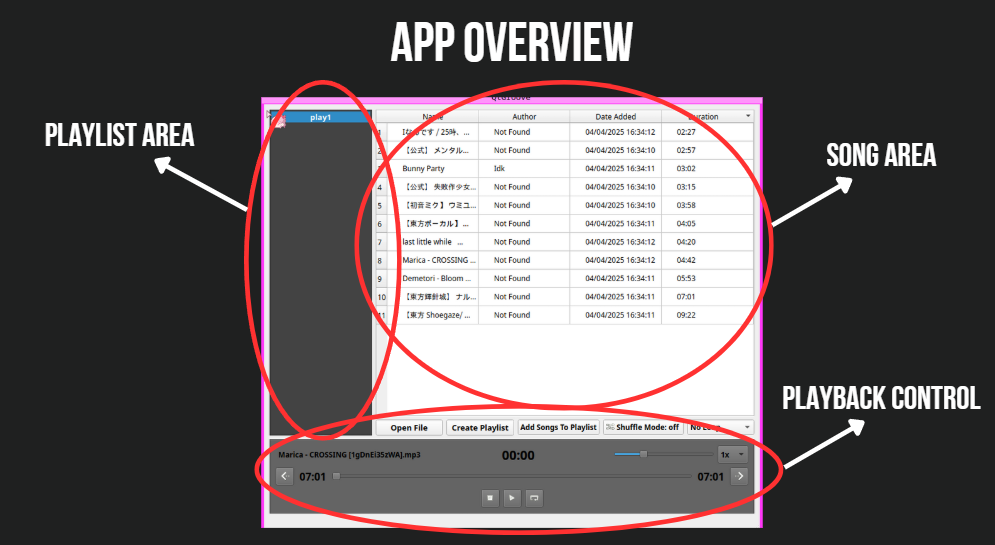
\includegraphics[width=0.6\textwidth]{images/app_overview.png} % Adjust width as needed

And here are our buttons.

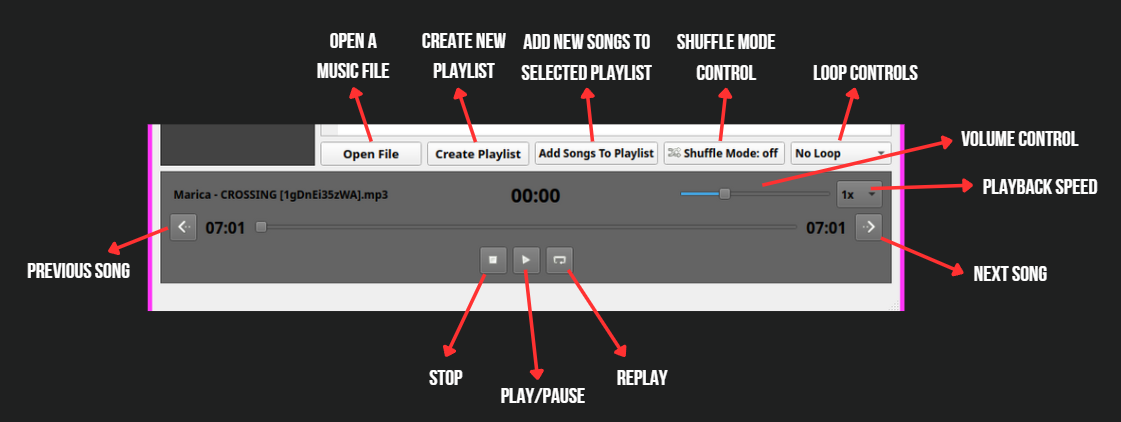
\includegraphics[height=0.25\textwidth]{images/btns.png} % Adjust width as needed

\newpage

\section{Database}

\hspace{1cm}We use SQLite for our database.

\subsection{playlist.db}

\hspace{1cm}We created playlist.db in the 'db' directory and that file will
be our main database file.

Our 'playlist.db' has default table named 'playlists' to keep track about our playlists'
existences

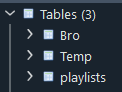
\includegraphics[width=0.7\textwidth]{images/tables.png} % Adjust width as needed

And in each playlists has their own columns which store the data.

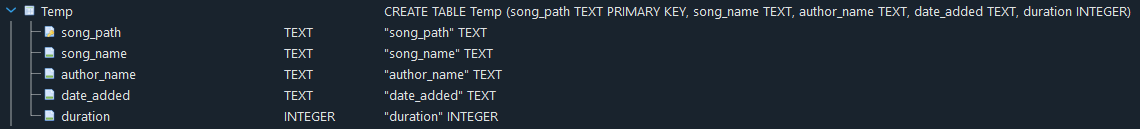
\includegraphics[height=0.1\textwidth]{images/cols.png} % Adjust width as needed

\newpage

\chapter{Installation and Execution Guide}
\section{Git Clone from the Remote Repository}
\begin{lstlisting}[language=Bash ,basicstyle=\footnotesize\ttfamily]
git clone https://github.com/Pottarr/QtGroove.git
\end{lstlisting}

After that open project in Qt Creator, and run the program.

\section{Alternative way for Windows users}

\hspace{1cm}You can download pre-release version (v0.1) from GitHub too.
(Link in Appendix)



% Chapter 4: Summary
\chapter{Summary}
\section{Learning Outcomes}
\begin{itemize}
    \item We have learnt fundamental of concepts of creating good UX and UI.
    \item We have learnt how to develop multi-platform application using C++ Qt.
    \item We have learnt the workflow of project developing.
    \item We have learnt how to use Version Control to help developing application.
\end{itemize}

\section{Accomplishment}
\hspace{1cm}We have created a user friendly multi-platform music player application.

\newpage

% References/Bibliography section
\chapter{References}
% Include your references here in the proper LaTeX format, or use a BibTeX file
\begin{itemize}
    \item Qt Group. (2025). \textit{Qt Documentation}. Retrieved from \url{https://doc.qt.io/}
\end{itemize}

\newpage

\chapter{Appendix}

\section{Github Repository}
\url{https://github.com/Pottarr/QtGroove}
% \newpage

\end{document}
